%% LyX 2.1.2 created this file.  For more info, see http://www.lyx.org/.
%% Do not edit unless you really know what you are doing.
\documentclass[british,compsoc,conference]{IEEEtran}
\usepackage[T1]{fontenc}
\usepackage[latin9]{inputenc}
\usepackage{float}
\usepackage{amsmath}
\usepackage{amssymb}
\usepackage{graphicx}
\usepackage{setspace}

\makeatletter

\newcommand{\noun}[1]{\textsc{#1}}

\@ifundefined{showcaptionsetup}{}{
 \PassOptionsToPackage{caption=false}{subfig}}
\usepackage{subfig}
\makeatother

\usepackage{babel}
\begin{document}

\title{Compositional design of asynchronous circuits \\
from behavioural concepts}
\author{Jonathan Beaumont, Andrey Mokhov, Danil Sokolov, Alex Yakovlev\\
\texttt{\{j.r.beaumont, andrey.mokhov, danil.sokolov, alex.yakovlev\}@ncl.ac.uk}\\
\emph{School of Electrical and Electronic Engineering, Newcastle University,
UK}}

\maketitle

\begin{abstract}
Asynchronous circuits can be useful in many applications, however,
they are yet to be widely used in industry. The main reason for this
is a steep learning curve for concurrency models, such Signal Transition
Graphs, that are developed by the academic community for specification
and synthesis of asynchronous circuits. In this paper we introduce
a compositional design flow for asynchronous circuits using \textit{concepts}
-- a set of formalised descriptions for system requirements. Our aim
is to simplify the process of capturing system requirements in the
form of a formal specification, and promote the concepts as a means
for design reuse. The proposed design flow is applied to the development
of an asynchronous buck converter. 
\end{abstract}

\sloppy
\thispagestyle{empty}\vspace{-2mm}



\section{Introduction}

\vspace{-2mm}


Asynchronous circuits are event-driven, i.e. they react to changes
in a system at the rate they occur~\cite{sparso2001principles}.
This makes them particularly useful for on-chip power management,
where the ability to quickly respond to dynamically changing loads
across the chip is essential for reliable operation and efficiency~\cite{2008_audy_isscc_tutorial}.
A power management system relies on analogue circuitry for power regulation
and conversion whose behaviour is characterised by many operating
modes and complexity of their interplay. Capturing all these aspects
of system behaviour in a consistent specification becomes the major
design challenge~\cite{2014_sokolov_ftfc}.

Signal Transition Graphs~(STGs) are commonly used for the specification
of asynchronous control circuits as they are compatible with multiple
synthesis tools, such as \noun{Petrify}~\cite{Cortadella} and \noun{Mpsat}~\cite{khomenko2004detecting}.
These tools take an STG specification of a complete controller and
produce a speed-independent circuit implementation~\cite{Muller_1959_ts}.
Such a monolithic approach to designing asynchronous circuits has
poor scalability: as the system grows in complexity its monolithic
specification becomes challenging to comprehend and debug. The STG
models of components cannot be reused when designing other specifications,
and thus each new design must be built from the ground up. This further
adds to the design time, hence making asynchronous circuits undesirable
for use in industry. 

To address this issue, we propose a new method of asynchronous circuit
design. The method splits a specification into several parts corresponding
to operational modes of the circuit (\emph{scenarios}). The features,
constraints and requirements of each scenario\emph{ }(\emph{concepts}),
are described in a formal notation, which we implemented as a domain
specific language embedded in Haskell~\cite{1996_hudak_dsl}. Concepts
can be composed and one concept can be made up of multiple smaller
concepts, thus supporting the design reuse at the level of system
specification. Scenarios of reconfigurable systems~\cite{microadapt}
can also be parameterised by run-time parameters (e.g., available
energy budget) or design-time ones (e.g., the number of processing
cores in a Network-on-Chip network), therefore concepts should also
support parameterisation.

A set of concepts describing the operation of a scenario is then passed
into a translation algorithm that automatically converts it into an
equivalent STG, which satisfies all given concepts and can be model-checked
using standard tools~\cite{2007_poliakov_workcraft}. When all scenarios
have been translated to STGs and verified, they can be combined to
produce a complete specification. This step will also be automated,
and will offer \emph{templates} for common scenario ordering requirements,
such as mode switching sequences and start-up scenarios. 



Designing a controller for an analogue circuit using this method can
be beneficial. Any of the partial knowledge we have about any casual
relationships between events in the environment can be naturally modelled
as concepts. When composed with other concepts describing these relationships
and concepts describing the control which reacts to the environment,
a model will be produced which shows how the environment and the control
system interacts. 



There are several existing methodologies which are similar to the
one being proposed in this paper, however we found them limited in
certain aspects as discussed below. 

\textbf{Snippets}~\cite{raey}, similar to concepts, are smaller
state graph models which are used to compose full state graphs of
larger systems. Snippets describe the operation of a part of a system
in terms of input and output alphabets, and in which ways these snippets
can fail. When composed with other snippets it can produce a working
system state graph model. With our design methodology however we want
to go deeper and decompose a component into concepts responsible for
capturing signal behaviours for system features, such as handshakes,
mutual exclusion, synchronisation, etc. 

\textbf{Structural design} features re-usability of modular components~\cite{modular-circuit-design}.
Here, a component design can be used multiple times across full device
designs in conjunction with several other circuit modules. These modules
can be changed in some way without affecting how they are used in
the full device designs. The ideas of this method are similar to that
of the design methodology we are proposing to reduce design time.
However, this method is at a much higher level, using fully designed
and tested components where as we propose to allow re-usability when
modelling at circuit level, using composed concepts. 

\textbf{DI algebra}~\cite{josephs1993overview} is a method of describing
systems as algebraic equations. Each equation represents an operation
of the specification, similar to scenarios, and composing these can
be simplified for the most compact version of the equation. These
can then be composed to find an equation for the whole specification
and again simplified for the most compact version. Our method is similar
to DI algebra, however concepts are described textually, which is
different to DI algebra and as such, simplification does not occur
at concept level, but during the composition and combination steps,
and the most compact form of the model is automatically produced.
To the best of our knowledge there are no tools or methodologies supporting
compositional design of asynchronous circuits using DI algebra and
it is therefore not interoperable with the rest of our design flow,
and this also makes it unsuitable for use in an industrial setting.

\textbf{Resynthesis}~\cite{Resynth2} is a process of decomposing
a full model and recomposing it of selective components to produce
a smaller model. This can be used to reduce the number of signals
to connect two separate models for example. This process is regularly
used for optimisation of Balsa control circuits~\cite{plana2005attacking},
however in Balsa the set of predefined components is fixed, so a designer
cannot easily introduce new scenarios. Resynthesis also requires full
models which can be decomposed. This requirement may be problematic
for the proposed methodology as we take a ground-up approach to composition,
starting with primitive concepts which composed into scenarios, which
are subsequently combined into a complete model. Resynthesis can still
be used at a later stage of the design process, once the complete
model of a system~(or a subsystem) has been obtained using the proposed
methodology. 

The idea is that our approach should reduce the complexity of designing
asynchronous circuits, so the number of errors should be reduced,
and easier to find and correct. This will in turn reduce the design
time, and make asynchronous circuits more desirable and be used to
make devices. 

The presented approach is automated in the open-source\noun{ Workcraft}
framework~\cite{2007_poliakov_workcraft}. This parses concepts,
uses them to produce scenario STGs and performs parallel composition~\cite{PCOMP}
on these and creates full model STGs. Full models can then be synthesised
using \noun{Workcraft}. In this paper, we use real life industrial
example of a buck converter~\cite{2014_sokolov_ftfc} to show our
design flow, and test this design approach. \vspace{-2mm}

\section{Motivating Example \label{sec:Motivating Example}}

Signal transition graphs are currently used for the specification of asynchronous circuits, and a monolithic design approach is used. This approach can become problematic however as designs become larger. In this section we will discuss this approach in detail and it's disadvantages. Following this, we will explore a way of viewing STGs which has helped us develop concepts.  

+ Here is the problem we are solving



+ STGs are a conventional specification model, STGs tend to get very large and complex for real-life circuits (show simple-buck example STG)



+ STGs mix many different concerns in one single graph -- show how one could split the specification into what we call concepts.

\section{Concepts \label{sec:Concepts}}

\vspace{-2mm}


In this section we formally introduce \emph{concepts} that we propose
to employ for the specification of asynchronous circuits. Below we
list (fairly standard) definitions and notational conventions that
are used throughout the paper.

We use $\mathbb{B}$ to denote the set of Boolean values $\{0,1\}$.
Given two Boolean functions $f:X\rightarrow\mathbb{B}$ and $g:X\rightarrow\mathbb{B}$
with the same domain $X$, we lift Boolean operators (disjunction~$\vee$,
conjunction~$\wedge$, implication $\Rightarrow$, etc.) in the usual
manner: $h=f\vee g$ means $h(x)=f(x)\vee g(x)$ for all $x\in X$,
etc. Furthermore,~$\mathbf{0}$ and~$\mathbf{1}$ stand for constant
Boolean functions that discard their input and return values $0$
and $1$, respectively.

A\emph{ monoid} is a set $M$ and a binary operation $\diamond:M\times M\rightarrow M$
satisfying two axioms:
\begin{itemize}
\item Identity: $e\diamond a=a\diamond e=a$ for any $a\in M$, where $e\in M$
is the \emph{identity element} of the monoid.
\item Associativity: $a\diamond(b\diamond c)=(a\diamond b)\diamond c$ for
all $a,b,c\in M$.
\end{itemize}
Monoid is the simplest mathematical structure that captures the notions
of \emph{emptiness} and \emph{composition}. The concepts introduced
in this section form \emph{commutative monoids}: they have identity
elements corresponding to empty specifications, and can be composed
to build complex concepts from simpler ones. The order of composition
does not matter, i.e., the concepts commute: $a\diamond b=b\diamond a$
for all $a,b\in M$. 

\vspace{-3mm}



\subsection{Abstract concepts}

\vspace{-3mm}


We first describe \emph{abstract concepts} that we use as building
blocks for developing \emph{domain specific concepts}, such as those
related to asynchronous circuits (Section~\ref{sub:Concepts-for-asynchronous}).


Abstract concepts are parameterised by finite sets of \emph{states}
$S$ and \emph{events} $E$. The \emph{initial state concept} captures
all possible (or \emph{permitted}) initial states of the system. In
the most general form it is a function
\[
\mathsf{initial}:S\rightarrow\mathbb{B}
\]
that given a state $s\in S$ returns $1$ if $s$ is an initial state
and $0$ otherwise. In practice this concept is often realised as
a membership test of a set of initial states~$I\subseteq S$, i.e.
$\mathsf{initial}(s)=s\in I$. However, we prefer the functional form
because it is more abstract and permits other, often more efficient
realisations. Note that~$\mathbf{0}$ and~$\mathbf{1}$ have natural
interpretations as initial concepts: they correspond to systems with
no initial states, and systems where any state can be initial, respectively.
Initial state concepts form a commutative monoid with the identity
element~$\mathbf{1}$ and the composition operation~$\wedge$. Intuitively,
if a system comprises two subsystems then its initial state should
satisfy constraints imposed by both subsystems, hence the conjunction
operator.

The \emph{event excitation concept} captures all states wherein a
given event can occur (or is \emph{excited}). In the most general
form it is a function
\[
\mathsf{excited}:E\times S\rightarrow\mathbb{B}
\]
that given an event $e\in E$ and a state $s\in S$ checks whether
$e$ is excited in $s$. In practice this concept is often realised
using \emph{interpreted graph models} such as Finite State Machines
and Petri Nets~\cite{Cortadella}, Conditional Partial Order Graphs~\cite{CPOG1},
and others. A partial application of the excitation function is often
useful: $\mathsf{excited}(e)$ captures all states where event $e$
is excited; for example, if $\mathsf{excited}(e)=\mathbf{0}$ then
$e$ is never excited or \emph{dead}. Event excitation concepts also
form a commutative monoid with~$e=\mathbf{1}$ and~$\diamond=\wedge$.
This definition corresponds to the \emph{parallel composition} operation,
a standard notion for many behavioural models~\cite{PCOMP}.

Some states may be impossible or undesirable during the normal system
operation. To express this we use the \emph{invariant concept}, which
captures all \emph{correct} or \emph{permitted} states of the system.
A typical use case for invariant concepts is to specify assertions
or assumptions about the system state space, that may by verified
via model checking and/or used for optimising the implementation.
In the most general form an invariant concept is a function
\[
\mathsf{invariant}:S\rightarrow\mathbb{B}
\]
that given a state $s\in S$ returns $1$ if $s$ is permitted by
the invariant and $0$ otherwise. Note that if for some state $s$
the initial concept $\mathsf{initial}(s)$ holds but the invariant
$\mathsf{invariant}(s)$ does not hold, then the specification is
\emph{contradictory} and cannot be satisfied by any implementation.
We therefore usually assume that $\mathsf{initial}(s)\Rightarrow\mathsf{invariant}(s)$
holds for all $s\in S$. Similarly, invariant concepts form a commutative
monoid with~$e=\mathbf{1}$ and~$\diamond=\wedge$. Intuitively,
if a system comprises two subsystems then its states should be permitted
in both of the subsystems. 





One can derive other useful concepts from the three concepts described
above, for instance, 
\[
\mathsf{quiescent}(e,s)=\overline{\mathsf{excited}(e,s)}
\]
captures all states $s\in S$ when a given event $e\in E$ cannot
occur. Furthermore, one can define other useful concepts that cannot
be derived from the above, e.g., the \emph{execution concept} capturing
the effects that different events have on the system state. Due to
space limitations we only consider the three concepts defined above
and their derivatives.

All described concepts form monoids, hence their combinations are
trivially monoids too. It is therefore convenient to consider triples
of concepts $(\mathsf{initial},\mathsf{excited},\mathsf{invariant})$
with $(\mathbf{1},\mathbf{1},\mathbf{1})$ representing the \emph{empty
specification}, and composition $(\mathsf{initial}_{1},\mathsf{excited}_{1},\mathsf{invariant}_{1})\diamond(\mathsf{initial}_{2},\mathsf{excited}_{2},\mathsf{invariant}_{2})$
defined as $(\mathsf{initial}_{1}\diamond\mathsf{initial}_{2},\mathsf{excited}_{1}\diamond\mathsf{excited}_{2},\mathsf{invariant}_{1}\diamond\mathsf{invariant}_{2})$.
Importantly, composition of two non-contradictory specifications is
always non-contradictory, that is if both $\mathsf{initial}_{1}(s)\Rightarrow\mathsf{invariant}_{1}(s)$
and $\mathsf{initial}_{2}(s)\Rightarrow\mathsf{invariant}_{2}(s)$
hold for all states $s\in S$, then $\mathsf{initial}_{1}(s)\diamond\mathsf{initial}_{2}(s)\Rightarrow\mathsf{invariant}_{1}(s)\diamond\mathsf{invariant}_{2}(s)$
holds too.

\vspace{-3mm}



\subsection{Concepts for asynchronous circuits\label{sub:Concepts-for-asynchronous}}

\vspace{-2mm}


We now introduce concepts which are specific for the domain of asynchronous
circuits and express them using the abstract concepts defined above. 

\textbf{Signal-level concepts:} States and events of an asynchronous
circuit are parameterised by a fixed set of signals $A$. A state
$s\in S$ is an assignment of Boolean values to signals, i.e. a function
$s:A\rightarrow\mathbb{B}$, while an event $e\in E$ is a \emph{signal
transition}, i.e. a pair $e:A\times\mathbb{B}$ comprising a signal
$a\in A$ and the value of the signal \emph{after} the transition
occurs. We call transitions $(a,0)$ and $(a,1)$ \emph{falling} and
\emph{rising}, respectively, and denote them by $a^{-}$ and $a^{+}$
for brevity.

The following two predicates are very useful for constructing concepts:
\[
\begin{array}{ccc}
\mathsf{before} & \!\!\!\!:\!\!\!\!\! & E\times S\rightarrow\mathbb{B}\\
\mathsf{after} & \!\!\!\!:\!\!\!\!\! & E\times S\rightarrow\mathbb{B}
\end{array}
\]
A state $s\in S$ is said to be \emph{before} a transition $(a,b)\in E$
if $s(a)\neq b$, i.e. in state $s$ signal $a$ has a value which
is different from the resulting value of the transition. Similarly,
$s$ is \emph{after} $(a,b)$ if $s(a)=b$ (the transition has already
occurred).

We are now ready to define an excitation concept called \emph{consistency}~\cite{Cortadella}:
\[
\mathsf{consistency}=\mathsf{before}
\]
This concept captures the requirement that in a consistent asynchronous
circuit a signal transition can only be excited in states that are
before it.

Another key concept in asynchronous circuits is \emph{causality}:
we say that a transition $\mathit{effect}\in E$ causally depends
on transition $\mathit{cause}\in E$, denoted as 
\[
\mathsf{causality}(\mathit{cause},\mathit{effect}):E\times S\rightarrow\mathbb{B}
\]
 if $\mathit{effect}$ can occur only in states that are after $\mathit{cause}$.
This is an excitation concept, which can be expressed as follows:
\[
\mathsf{causality}(\mathit{cause},\mathit{effect})(e)\!=\!\begin{cases}
\mathbf{1} & \mathit{if}\, e\neq\mathit{effect}\\
\mathsf{after}(cause) & \mathit{otherwise}
\end{cases}
\]
In words, we do not add any constraints to events $e\in E$ that are
distinct from $\mathit{effect}$, but $\mathit{effect}$ is constrained
to occur only after $\mathit{cause}$. Note that function $\mathsf{after}$
is used in the partially applied form. We will use a short-hand notation
\[
\mathit{cause}\rightsquigarrow\mathit{effect}
\]
for the causality concept for convenience.

One can compose two causality concepts using the monoid composition,
for example
\[
a\rightsquigarrow c\ \diamond\ b\rightsquigarrow c
\]
corresponds to so-called AND-causality: event $c$ can only occur
after both $a$ and $b$ have occurred. Specifying OR-causality is
slightly more tricky:
\[
\mathsf{orCausality}(a,b,c)(e)=\begin{cases}
\mathbf{1} & \mathit{if}\, c\neq\mathit{e}\\
\mathsf{after}(a)\vee\mathsf{after}(b) & \mathit{otherwise}
\end{cases}
\]
Event $c$ is thus excited after at least one cause has occurred.

\textbf{Gate-level concepts:} Using the causality concept we can express
the behaviour of gates in asynchronous circuits. For example, a \emph{buffer}
is a gate with one input signal $a\in A$ and one output signal $b\in A$,
whose output transitions causally depend on the input ones:
\[
\mathsf{buffer}(a,b)=a^{+}\rightsquigarrow b^{+}\ \diamond\ a^{-}\rightsquigarrow b^{-}
\]
An \emph{inverter} has a similar conceptual specification, but the
output transition is inverted:
\[
\mathsf{inverter}(a,b)=a^{+}\rightsquigarrow b^{-}\ \diamond\ a^{-}\rightsquigarrow b^{+}
\]
A \emph{C-element} is a gate with two inputs $a$ and $b$ and one
output~$c$, which synchronises input transitions:
\[
\mathsf{cElement}(a,b,c)=a^{+}\!\rightsquigarrow\! c^{+}\ \diamond\ b^{+}\!\rightsquigarrow\! c^{+}\ \diamond\ a^{-}\!\rightsquigarrow\! c^{-}\ \diamond\ b^{-}\!\rightsquigarrow\! c^{-}
\]
In words, the rising output transition $c^{+}$ causally depends on
both $a^{+}$ and $b^{+}$, and the falling output transition $c^{-}$
causally depends on both $a^{-}$ and $b^{-}$. An alternative way
to express the same concept is to reuse the buffer concept:
\[
\mathsf{cElement}(a,b,c)=\mathsf{buffer}(a,c)\ \diamond\ \mathsf{buffer}(b,c)
\]
Indeed, a C-element combines the constraints imposed on the output
transitions by two `virtual' buffers.

Behaviour of other gates can be similarly defined using concepts,
see our Haskell implementation~\cite{2015_concepts_github}.

\textbf{Protocol-level concepts:} In addition to gate-level concepts
described above it is often important to specify \emph{protocols}
of interaction between multiple gates or components. In this section
we demonstrate how one can use concepts to specify asynchronous handshakes
and mutual exclusion mechanisms.

Given two signals $a$ and $b$, a \emph{handshake} between them is
the following composition of causality concepts:
\[
\mathsf{handshake}(a,b)=a^{+}\!\rightsquigarrow\! b^{+}\ \diamond\ b^{+}\!\rightsquigarrow\! a^{-}\ \diamond\ a^{-}\!\rightsquigarrow\! b^{-}\ \diamond\ b^{-}\!\rightsquigarrow\! a^{+}
\]
Intuitively, we have a two-way asynchronous communication channel,
where one party sends transitions $a^{+}$ and $a^{-}$ and the other
party responds by corresponding $b^{+}$ and $b^{-}$ transitions.
One can notice that the four causality concepts match those found
in the buffer and inverter concepts, which leads to an alternative
way to express a handshake between~$a$ and~$b$:
\[
\mathsf{handshake}(a,b)=\mathsf{buffer}(a,b)\diamond\mathsf{inverter}(b,a)
\]
Indeed, this conceptual understanding of a handshake as being composed
from a buffer and an inverter is often used by circuit designers as
a convenient way of reasoning. 

In order to specify the initial state of a handshake between signals~$a$
and~$b$, we can use functions $\mathsf{before}$ and $\mathsf{after}$.
For example, $\mathsf{before}(a^{+})$ captures the states where signal
$a$ is set to $0$. We can compose an initial state concept with
the handshake concept as follows:
\[
\mathsf{handshake00}(a,b)\!=\!\mathsf{handshake}(a,b)\diamond\mathsf{before}(a^{+})\diamond\mathsf{before}(b^{+})
\]
The resulting concept corresponds to a handshake between signals~$a$
and~$b$ that are both initially $0$.

The last important concept that requires an introduction is \emph{mutual
exclusion} between two signals~$a$ and~$b$:
\[
\mathsf{me}(a,b)=a^{-}\rightsquigarrow b^{+}\ \diamond\ b^{-}\rightsquigarrow a^{+}\diamond\overline{\mathsf{after}(a^{+})\wedge\mathsf{after}(b^{+})}
\]
The concept comprises two parts: 1) in terms of causality, we say
that rising transitions $a^{+}$ and $b^{+}$ can only occur after
the opposite falling ones, 2) the initial states when $a=b=1$ are
forbidden. Taken together these two parts guarantee that $a$ and
$b$ are never set to $1$ at the same time, i.e. they are mutually
exclusive. We also add $\overline{\mathsf{after}(a^{+})\wedge\mathsf{after}(b^{+})}$
to the invariant.

We can now specify a \emph{mutual exclusion element}~\cite{2008_kinniment_synchronisation}
that receives asynchronous requests $r_{1}$ and $r_{2}$ to a shared
resource and grants access to it by corresponding mutually exclusive
signals $g_{1}$ and $g_{2}$:

\vspace{-3mm}
{\small{}
\[
\mathsf{meElement}(r_{1},r_{2},g_{1},g_{2})\!=\mathsf{\! buffer}(r_{1},g_{1})\diamond\mathsf{buffer}(r_{2},g_{2})\diamond\mathsf{me}(g_{1},g_{2})
\]
}{\small \par}

\vspace{-3mm}

\subsection{Signal types}

A discussion of signal types and how these are represented using concepts. The benefits of this, for example we can block input -> input. 

\section{Circuit specification with concepts \label{sec:Circuit-specification-with}}

\vspace{-2mm}




This section presents a method for deriving a circuit specification
from a set of concepts that describe its different aspects. We focus
on specification of \emph{Speed-Independent}~(SI) circuits, which
is an important class of asynchronous circuits~\cite{Muller_1959_ts}
that work correctly regardless of the gates' delays, while the wires
are assumed to have negligible delays. Alternatively, one can regard
wire forks as isochronic and add wire delays to the corresponding
gate delays~(\emph{Quasi-Delay Insensitive}~(QDI) circuit class~\cite{Martin_1986_dc}).
A convenient formalism for specification of SI circuits is STGs~\cite{Chu_1987_phd,Rosenblum_1985_tpn},
which is a special kind of Petri nets~\cite{Petri_1962_phd} whose
transitions are associated with signal events. 

\vspace{-3mm}



\subsection{Petri nets and STGs}

\vspace{-3mm}


Formally, a Petri net is defined as a tuple~$PN=\left\langle P,\, T,\, F,\, M_{0}\right\rangle $
comprising finite disjoint sets of \emph{places~}$P$ and \emph{transitions~}$T$,
\emph{arcs} denoting the flow relation~$F\subseteq\left(P\times T\right)\cup\left(T\times P\right)$
and \emph{initial~marking~}$M_{0}$. There is an arc between~$x\in P\cup T$
and~$y\in P\cup T$ iff $\left(x,y\right)\in F$. The \emph{preset}
of a node $x\in P\cup T$ is defined as $\bullet x=\left\{ y\mid\left(y,x\right)\in F\right\} $,
and the \emph{postset} as $x\bullet=\left\{ y\mid\left(x,y\right)\in F\right\} $.
The dynamic behaviour of a Petri net is defined as a \emph{token~game},
changing marking according to the enabling and firing rules. A \emph{marking}
is a mapping~$M:\, P\rightarrow\mathbb{N}$ denoting the number of
\emph{tokens} in each place~($\mathbb{N}=\left\{ 0,1\right\} $ for
\emph{1-safe} Petri nets). A transition $t$ is \emph{enabled} iff
$\forall p,p\in\bullet t\Rightarrow M(p)>0$. The evolution of a Petri
net is possible by \emph{firing} the enabled transitions. \emph{Firing}
of a transition~$t$ results in a new marking $M'$ such that 
\[
M'\left(p\right)=\left\{ \begin{array}{cc}
M(p)-1 & if\, p\in\bullet t\setminus t\bullet,\\
M(p)+1 & if\, p\in t\bullet\setminus\bullet t,\\
M(p)\,\,\,\,\, & otherwise
\end{array}\right.
\]
 for all $p\in P$. 

An STG is a 1-safe Petri net whose transitions are labelled by signal
events, i.e. $STG=\left\langle P,\, T,\, F,\, M_{0},\,\lambda,\, Z,\, v_{0}\right\rangle $,
where $\lambda$ is a \emph{labelling~function}, $Z$ is a set of
\emph{signals} and $v_{0}\in\left\{ 0,\,1\right\} ^{\left|Z\right|}$
is a \emph{vector~of}~\emph{initial~signal~values}. The labelling
function $\lambda:T\rightarrow Z\pm$ maps transitions into \emph{signal~events}
$Z\pm=Z\times\left\{ +,-\right\} $. The signal events labelled $z+$
and $z-$ denote the transitions of signals $z\in Z$ from 0~to~1~(rising
edge), or from 1~to~0~(falling edge), respectively. The labelling
function does not have to be 1-to-1, i.e. transitions with the same
label may occur several times in the net. To distinguish transitions
with the same label and refer to them from the text an index $i\in\mathbb{N}$
is attached to their labels as follows: $\lambda\left(t\right)/i$,
where $i$ differs for different transitions with the same label.
STGs inherit the operational semantics of their underlying PNs, including
the notions of transition enabling and firing.

Graphically, the places are represented as circles, transitions as
text labels, consuming and producing arcs are shown by arrows, and
tokens are depicted by dots. For simplicity, the places with one incoming
and one outgoing arc are often hidden, allowing arcs~(with implicit
places) between transitions.

\vspace{-3mm}



\subsection{Composition of concepts}

\vspace{-3mm}


A single concept can be used to describe an initial state, invariant
states, a single event or a combination of these, yet describing some
protocols using this method can become long winded, as these can involve
multiple events. We make use of the monoid composition of concepts
to describe complex systems incrementally. Importantly we can mix
several levels of system description and refer to signal, gate and
protocol level concepts in one specification, depending on which level
is more convenient in a particular situation. 

Consider a C-element example whose signals $a$ and $b$ are inputs,
and signal $c$ is the output. When input $a$ or $b$ changes, we
assume it remains in the new state until the output $c$ changes.
The following signal-level concepts describe this system: 

\vspace{2mm}
\begin{minipage}[t]{1\columnwidth}%
\begin{flushleft}
$\,\mathsf{outputRise}=a^{+}\rightsquigarrow c^{+}\,\diamond\, b^{+}\rightsquigarrow c^{+}$
\par\end{flushleft}

\begin{flushleft}
$\,\mathsf{inputFall}=c^{+}\rightsquigarrow a^{-}\,\diamond\, c^{+}\rightsquigarrow b^{-}$
\par\end{flushleft}

\begin{flushleft}
$\,\mathsf{outputFall}=a^{-}\rightsquigarrow c^{-}\,\diamond\, b^{-}\rightsquigarrow c^{-}$
\par\end{flushleft}

\begin{flushleft}
$\,\mathsf{inputRise}=c^{-}\rightsquigarrow a^{+}\,\diamond\, c^{-}\rightsquigarrow b^{+}$
\par\end{flushleft}

\begin{flushleft}
$\,\mathsf{initialState}=\mathsf{before}(a^{+})\,\diamond\,\mathsf{before}(b^{+})\,\diamond\,\mathsf{before}(c^{+})$
\par\end{flushleft}

\begin{flushleft}
$\begin{aligned}\mathsf{system}= & \mathsf{\, outputRise}\,\diamond\,\mathsf{inputFall}\,\diamond\,\mathsf{outputFall\,\diamond}\\
 & \mathsf{\, inputRise}\,\diamond\,\mathsf{initialState}
\end{aligned}
$
\par\end{flushleft}%
\end{minipage}\vspace{2mm}


There are 6 concepts featured, the first 5 of which describe certain
operations of the system. The sixth concept composes all of the first
5 concepts, and can be translated to the STG shown in Figure~\ref{fig:cElement STG}.
The first four are named according to what they represent, for example,
\textsf{\textit{\emph{outputRise}}}\textit{ }describes the events
which cause the output to rise\textit{.} The fifth concept is the
initial state concept. This is necessary for the algorithm to produce
a scenario STG, as the STG produced will not be usable without knowing
the states the signals will be in when the scenario is entered. The
algorithm takes this concept and works out where tokens need to be
placed in the STG produced. 

\begin{figure}[h]
\begin{centering}
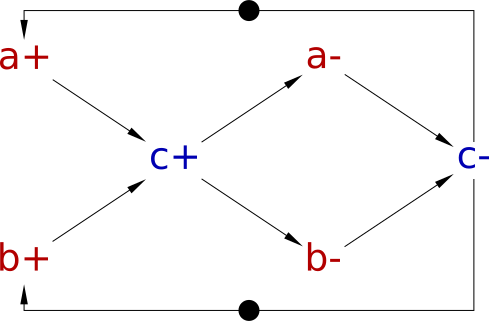
\includegraphics[scale=0.23]{Images/stg-cElement}
\par\end{centering}

\protect\caption{\label{fig:cElement STG}STG for the example system.}
\end{figure}


This set of concepts is only one way of describing this C-element
and the environment. Another way could be to use gate-level concepts
and describe the environment explicitly. In this case the environment
allows the inputs to transition in the opposite direction to the output
$c$, as two inverters would. We can then compose this with the C-element
and the same initial state concept:\vspace{1mm}


\begin{minipage}[t]{1\columnwidth}%
$\mathsf{environment}=\mathsf{inverter}(c,a)\,\diamond\,\mathsf{inverter}(c,b)$

$\mathsf{system}=\mathsf{cElement}(a,b,c)\,\diamond\,\mathsf{environment}\,\diamond\,\mathsf{initialState}$%
\end{minipage}\vspace{2mm}
This specification is equivalent to the previous one; indeed one can
prove this by rearranging the primitive concepts using the commutativity
and associativity axioms of the underlying commutative monoid. Consequently,
this specification will be translated to the same STG shown in Figure~\ref{fig:cElement STG}.
Figure~\ref{fig:cElement-concepts} illustrates all the concepts
involved in this specification.

\begin{figure}[t]
\begin{centering}
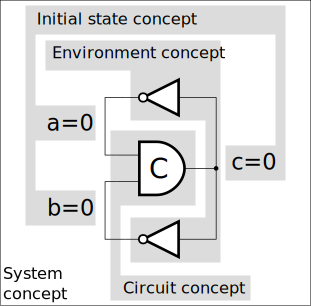
\includegraphics[scale=0.6]{Images/c-element-circuit}
\par\end{centering}

\protect\caption{\label{fig:cElement-concepts}Example system specified using concepts.}
\end{figure}


Finally, the designer can also rely on protocol-level concepts, producing
the following equivalent specification:\vspace{1mm}


\begin{minipage}[t]{1\columnwidth}%
$\mathsf{system}=\mathsf{handshake00}(a,c)\,\diamond\,\mathsf{handshake00}(b,c)$%
\end{minipage}\vspace{2mm}
This example demonstrates that the presented formal notation for capturing
concepts is very flexible and provides the designer with a rich selection
of available levels of abstraction, which could be used not only for
deriving simplest possible specifications but also for cross-checking
the adequacy of specifications by \emph{refactoring} them according
to the composition laws.

\vspace{-3mm}



\subsection{Multiple behavioural scenarios}

\vspace{-2mm}


So far we have only considered systems operating in a single behavioural
\textit{scenario} specified by a composition of concepts. However,
real-life systems often need to support multiple scenarios~ (e.g.,
start-up and normal operation, different power modes~\cite{microadapt},
etc.). This allows each individual scenario to be designed using concepts,
and tested individually to ensure they work correctly, before these
are combined to produce a full system specification. 

To increase the re-usability of scenarios, which helps reduce design
time of future systems, this method supports the use of pre-designed
scenarios as concepts. 

In some cases, a designer may find it easier to split the specification
of operational modes further than scenarios and design certain elements
separately. In this way, a model may be produced from concepts, which
may not be an operational mode on its own, but can be composed and
tested separately. In some cases, having several elements predefined
using concepts may become useful for quickly designing systems. A
predefined logic gate, for example, could be useful to include quickly
in any list of concepts when designing multiple scenarios. An STG
produced of this element can be referenced in a list of concepts by
name (provided that the definition is appropriately imported into
the current namespace). When a list of concepts is passed into the
STG translation algorithm, all referenced concepts are replaced by
the corresponding definitions. 

\vspace{-3mm}


\section{Interoperability with STG based tools \label{sec: interop-with-stg}}

+ Algorithm for converting concepts to STGs

+ Using parallel and scenario composition to produce STGs for the whole system

+ Direct synthesis from concepts
\section{NEED TO REMOVE: Synthesis of STGs from concepts \label{sec:Synthesis-of-STGs}}

\vspace{-3mm}
\textbf{This section needs to be edited to be included in section \ref{sec: interop-with-stg}}

\vspace{5mm}

When a list of concepts is produced, we then pass this into an algorithm
which converts these into a single scenario STG that, if possible,
satisfies all of the concepts. This STG represents one operational
mode of a full specification, and this needs to be combined with other
scenario STGs in order to produce a full system specification. In
this section we will discuss how this process is performed, from concepts,
to a set of scenario STGs, to a full system model. 

\vspace{-2mm}



\subsection{Deriving STG fragments from concepts}

\vspace{-2mm}


The algorithm begins by expanding any predefined concepts, and this
returns a full list of concepts. Each concept can then be converted
into its own STG fragment. In some cases, a single concept can represent
a single STG fragment, but if a one-to-many concept is used, multiple
fragments can be produced. These fragments are all created and stored
for use in the next step, but hidden from the user. However, how the
fragments are produced is important. For example, an STG fragment
converted from the concept \textsf{\textit{\emph{outputRise}}} in
the above C-element example is shown in Figure~\ref{fig:outputRise STG}. 

\begin{figure}[h]
\begin{centering}
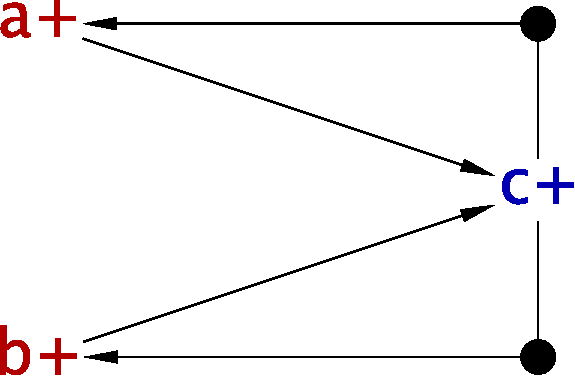
\includegraphics[scale=0.23]{Images/outputRise-stg}
\par\end{centering}

\protect\caption{\label{fig:outputRise STG}STG for the \textsf{\textit{\emph{outputRise}}}
concept.}
\end{figure}


This STG features arcs which suggest that \textsf{$a^{+}$} and $b^{+}$
must occur before \textsf{$c^{+}$}, as the concept suggests. This
fragment can also be seen as part of the scenario STG in Figure~\ref{fig:cElement STG}.
This concept however features two back-pressure arcs which are not
necessarily described in the concept. In order for fragments created
from concepts to be usable in producing scenario STGs, they need to
be complete, meaning they must have initial states, displayed using
tokens, and must not reach deadlock at any point, and this STG would
be incomplete without these back-pressure arcs used to show initial
states. These arcs are produced automatically by the algorithm, and
these fragments may be hidden from the user. 

\vspace{-3mm}



\subsection{Scenario STGs}

\vspace{-2mm}


If all concepts can be correctly converted into STG fragments, then
they can then be used to produce the STG for the scenario. This process
is done using a tool integrated in \noun{Workcraft} called \noun{Pcomp~}\cite{PCOMP},
which is designed to compose multiple STGs. The algorithm will automatically
take all STG fragments and pass them into the \noun{Pcomp} tool, and
this returns a single STG, created by composing all of the fragments.
It is necessary for all STG fragments to be complete, for example
using back-pressure arcs and including the initial states, as this
is used in the parallel composition process. 

We can use this process to produce STGs for scenarios, which are then
verified and simulated in \noun{Workcraft} and used in the next step.
However, if this STG is not to be used as a scenario but as a predefined
concept, this can be verified and stored for further use as part of
scenario descriptions. 

\vspace{-3mm}



\subsection{Combination of scenarios \label{sub:Combination-of-scenarios}}

\vspace{-3mm}


When a scenario STG has been produced and verified, it can then be
combined with other scenarios to produce a complete circuit specification.

When combining scenarios, there are several things to consider in
how the scenarios fit together. Depending on the application the circuit
is being designed for, some scenarios may need to operate in certain
orders, for example, one scenario may exist simply to initialise the
circuit, therefore this scenario needs to run at start-up, before
any of the other scenarios, and then never be run again while the
system remains active. 

To address this, when combining scenarios we offer some templates,
each of which can be used to combine scenarios in various orders.
With this the designer specifies in which ways the scenarios should
be combined, and if an order is needed, the order the scenarios should
be run from start up. The following are some examples of templates
that will be offered before scenarios are combined:

\textbf{Sequential:} Sequential combination will allow a designer
to select the order of all scenarios, so when combined, they will
run in a sequence. In this case, there may be a clear order in which
the scenarios may run, and this needs to be specified by the designer. 

\textbf{Concurrent:} In this case there is no order, but one or more
of the scenarios in a specification may run in parallel. This template
will combine the scenarios in a way that will allow concurrency to
occur, limited to requirements of the specification, for instance,
the number of scenarios that can be active at any one time, which
can be limited by the number of tokens available at once. 

\textbf{Non-deterministic choice:} This template will combine the
scenarios in a way that allows any of the scenarios to run, but not
according to any order to deal with the lack of determinism in the
system, using one token which is used only by the running scenario,
and this is returned when the scenario completes. 

There may be some more complex requirements to combination, and it
is possible to combine some scenarios using one template, then including
the result in a combination using another template. For example, a
system which is non-deterministic may also have a scenario that runs
at start up to initialise the system. In this case, a designer could
combine all non-deterministic scenarios first, then combine the resulting
STG with the initialising scenario, setting the order so this runs
first. 

This method of combination can allow for many possible scenario combination
styles, and more complex systems can be combined automatically, which
in comparison to manual combination, could reduce the number of errors
as well as design time. 

\vspace{-3mm}



\section{Case study}

\vspace{-2mm}


In this section we follow a case study to show the design flow of
this method using an example from power management domain~\cite{2014_sokolov_ftfc}.
A basic power regulator comprises an analogue buck and a digital controller,
as shown in Figure~\ref{fig:buck-schematic}. The controller operates
the power regulating PMOS and NMOS transistors of the buck~(using\textsf{
$gp$} and $gn$ outputs) as a reaction to \emph{under-voltage}~(UV),
\emph{over-current}~(OC) and \emph{zero-crossing}~(ZC) conditions~(\textsf{$uv$,}
\textsf{$oc$} and \textsf{$zc$} inputs, respectively). These conditions
are detected and signalled by a set of specialised sensors implemented
as comparators of measured current and voltage levels against some
reference values~(\textsf{V\_ref}, \textsf{I\_max}, \textsf{V\_0}).
Note that the $gp$ and $gn$ signals are buffered to drive the very
large power regulating transistors and their effect on the buck can
be significantly delayed. Therefore, the controller is explicitly
notified~(by the $gp\_ack$ and $gn\_ack$ signals) when the power
transistor threshold levels~(\textsf{Th\_pmos} and \textsf{Th\_nmos})
are crossed.

\begin{figure}[h]
\begin{centering}
\subfloat[\label{fig:buck-schematic}Schematic.]{\begin{centering}
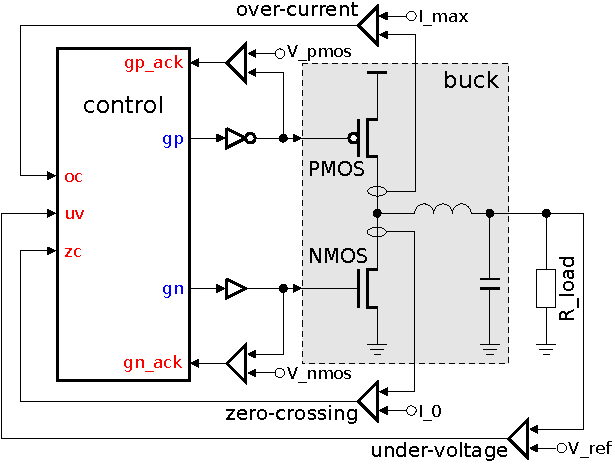
\includegraphics[scale=0.75]{Images/schematic-buck}
\par\end{centering}

}
\par\end{centering}

\begin{centering}
\subfloat[\label{fig:buck-spec}Informal specification.]{\begin{centering}
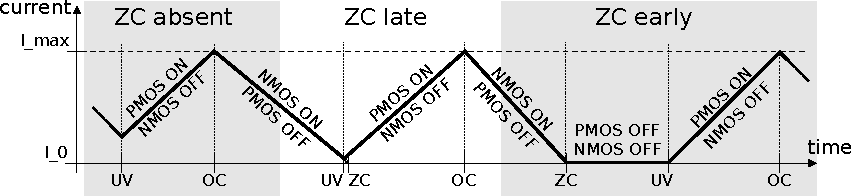
\includegraphics[scale=0.6]{Images/spec-buck}
\par\end{centering}

}
\par\end{centering}

\protect\caption{\label{fig:buck}Buck converter.}
\end{figure}


The operation of a power regulator is usually specified in an intuitive,
but rather informal way, e.g. by enumerating the possible sequences
of detected conditions and describing the intended reaction to these
events, as shown in Figure~\ref{fig:buck-spec}. The diagram shows
that UV should be handled by switching the NMOS transistor \noun{Off}
and PMOS transistor \noun{On}, while OC should revert their state~--
PMOS \noun{Off} and NMOS \noun{On}~(no~ZC scenario). Detection of
the ZC after UV does not change this behaviour~(late~ZC scenario).
However, if ZC is detected before UV then both the PMOS and NMOS transistors
remain \noun{Off} until the UV condition~(early~ZC scenario). 

Note that ZC and UV are independent conditions that indicate separate
physical effects and therefore the corresponding signals can happen
in any order. UV indicates that the voltage supplied to the load has
decreased below the reference value. ZC occurs when the coil current
reduces to~0 and causes the NMOS transistor to switch \noun{Off},
so that the NMOS acts like a diode and only conducts in one direction. 



\vspace{-3mm}



\subsection{Formal specification}

\vspace{-3mm}


From the informal buck specification and our knowledge of the signals,
we can determine three separate operating conditions that occur in
the analogue circuit and the controller needs to react to. All of
these can be produced from concepts separately and composed to produce
scenario STGs, before combining these to produce a single full circuit
STG. 

During this process, it is useful to find any operations which occur
between two or more operational modes, as these can then be reused
in other scenarios. If this is defined in one list of concepts, it
can then be referenced in concept lists for other scenarios by name. 


\subsubsection{No ZC scenario}

We start with describing the operational mode where no ZC condition
is signalled and produce the following list of concepts:

\begin{minipage}[t]{1\columnwidth}%
\begin{flushleft}
$\,\mathsf{uvFunc}=uv^{+}\rightsquigarrow gp^{+}\,\diamond\, uv^{+}\rightsquigarrow gn^{-}$
\par\end{flushleft}

\begin{flushleft}
$\,\mathsf{ocFunc}=oc^{+}\rightsquigarrow gp^{-}\,\diamond\, oc^{+}\rightsquigarrow gn^{+}$
\par\end{flushleft}

\begin{flushleft}
$\,\mathsf{uvReact}=gp\_ack^{+}\rightsquigarrow uv^{-}\,\diamond\, gn\_ack^{+}\rightsquigarrow uv^{-}$
\par\end{flushleft}

\begin{flushleft}
$\,\mathsf{ocReact}=gp\_ack^{-}\rightsquigarrow oc^{-}\,\diamond\, gn\_ack^{+}\rightsquigarrow oc^{-}$
\par\end{flushleft}

\begin{flushleft}
$\,\mathsf{environmentConstraint}=\mathsf{me}(uv,\, oc)$
\par\end{flushleft}

\begin{flushleft}
$\,\mathsf{\mathsf{circuitConstraint}}=\mathsf{me}(gn,\, gp)$
\par\end{flushleft}

\begin{flushleft}
$\,\mathsf{gpHandshake}=\mathsf{handshake}(gp,\, gp\_ack)$
\par\end{flushleft}

\begin{flushleft}
$\,\mathsf{gnHandshake}=\mathsf{handshake}(gn,\, gn\_ack)$
\par\end{flushleft}

\begin{flushleft}
$\,\mathsf{initialState}=\mathsf{before}(uv^{+})\,\diamond\,\mathsf{before}(oc^{+})$~
\par\end{flushleft}

\begin{flushleft}
$\begin{aligned}\mathsf{chargeFunc}= & \,\mathsf{ocFunc}\,\diamond\,\mathsf{ocReact}\,\diamond\\
 & \mathsf{\mathsf{\, environmentConstraint}\,\diamond\, circuitConstraint}\,\diamond\,\\
 & \mathsf{\, gpHandshake}\,\diamond\,\mathsf{gnHandshake}\,\diamond\,\mathsf{initialState}
\end{aligned}
$
\par\end{flushleft}

\begin{flushleft}
$\,\mathsf{zcAbsent}=\mathsf{quiescent}(zc^{+})\,\diamond\,\mathsf{quiescent}(zc^{-})$
\par\end{flushleft}

\begin{flushleft}
$\begin{aligned}\mathsf{zcAbsentScenario}= & \,\mathsf{chargeFunc}\,\diamond\,\mathsf{uvFunc}\,\diamond\,\mathsf{uvReaction}\,\diamond\\
 & \,\mathsf{zcAbsent}
\end{aligned}
$
\par\end{flushleft}%
\end{minipage}

\begin{flushleft}
\begin{figure}[H]
\begin{centering}
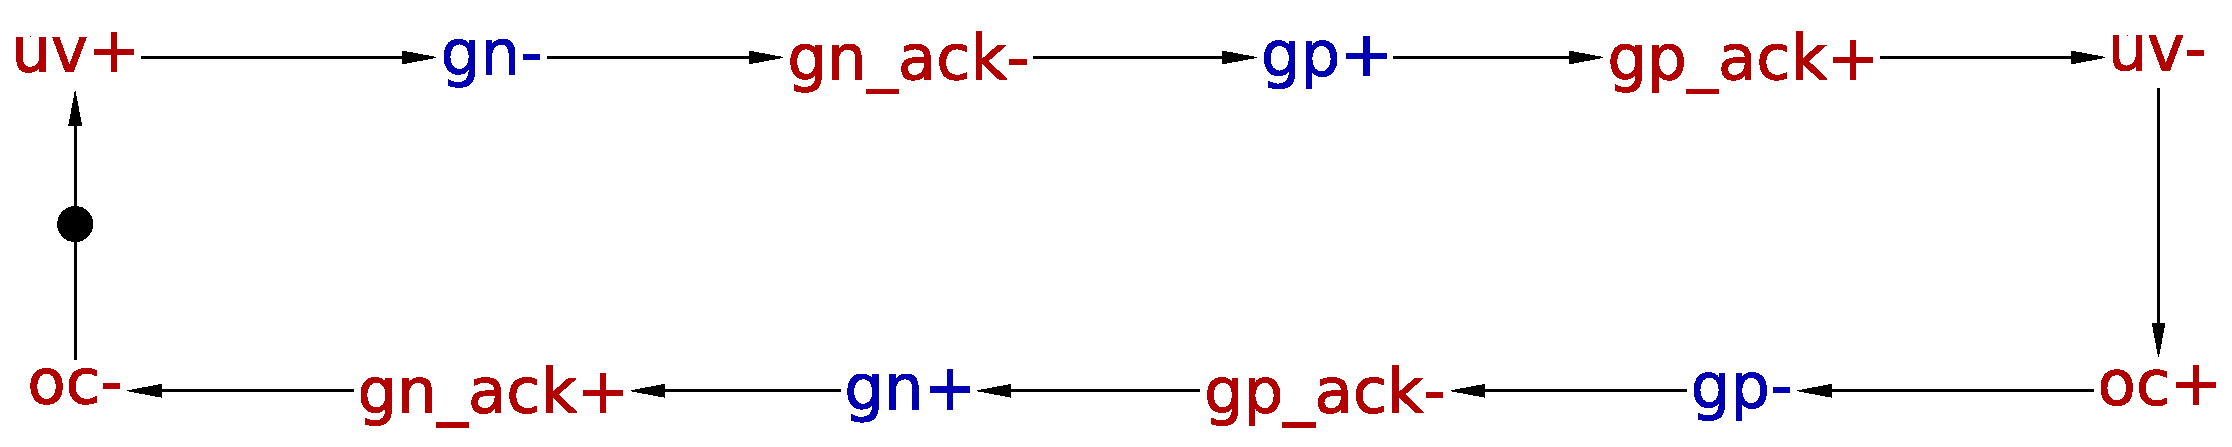
\includegraphics[scale=0.23]{Images/stg-UV_without_ZC}
\par\end{centering}

\protect\caption{\label{fig:zcAbsentScenario STG} STG for the \textsf{zcAbsentScenario}
concept.}
\end{figure}

\par\end{flushleft}

In this list, we introduce concepts which describe the correction
of both under-voltage and over-current. This includes concepts describing
handshakes for $gp/gp\_ack$ and $gn/gn\_ack$, and transistor safety
constraints which are described using protocol-level concepts. We
also describe constraints provided by the environment that we are
aware of, so this behaviour is captured in the resulting STG. 

The descriptions of the operational modes suggest that there are similarities
between them, mainly in the sequence of PMOS/NMOS activation during
the charging cycle. Therefore it is natural to define a \textsf{chargeFunc}
concept that can be reused when other operation modes are specified. 

Figure~\ref{fig:zcAbsentScenario STG} shows the STG produced from
the final concept in the list, \textsf{zcAbsentScenario}. It contains
two tokens which are created based on the \textsf{initialState} concept.
The analogue circuit is not guaranteed to signal either under-voltage
or over-current first, and this needs to be noted in the concepts
and the STG. 


\subsubsection{Late ZC scenario}

In this operational mode we have to include zero-crossing, as per
the specification. However, in this case under-voltage and over-current
are corrected in the same way as in the no~ZC scenario, and therefore
we can include the \textsf{zcAbsentScenario} concept. We still need
to describe the interactions involving zero-crossing. The concepts
are as follows:

\begin{minipage}[t]{1\columnwidth}%
\begin{flushleft}
$\,\mathsf{zcLate}=uv^{+}\rightsquigarrow zc^{+}\,\diamond\, zc^{-}\rightsquigarrow uv^{+}$
\par\end{flushleft}

\begin{flushleft}
$\begin{aligned}\mathsf{zcLateScenario}= & \mathsf{\, chargeFunc}\,\diamond\,\mathsf{uvFunc}\,\diamond\,\mathsf{uvReact}\,\diamond\\
 & \,\mathsf{zcLate}\,\diamond\,\mathsf{before}(zc^{+})
\end{aligned}
$
\par\end{flushleft}%
\end{minipage}

\begin{figure}[H]
\begin{centering}
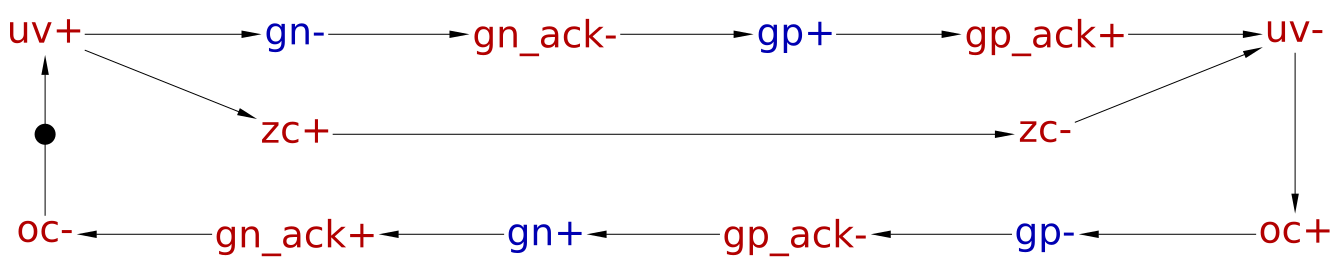
\includegraphics[scale=0.23]{Images/stg-UV_before_ZC}
\par\end{centering}

\protect\caption{\label{fig:zcLateScenario STG}STG for the \textsf{zcLateScenario}
concept.}


\end{figure}


Figure~\ref{fig:zcLateScenario STG} shows the STG produced, which
looks similar to the STG in Figure~\ref{fig:zcAbsentScenario STG}
but this features a branch from some $uv$ and $zc$ interaction.
This is defined in the concept \textsf{zcLateScenario}, which does
not describe the arc $zc^{+}\rightsquigarrow zc^{-}$ but this consistency
is implied in concepts, as for obvious reasons, $zc^{+}$ must occur
before $zc^{-}$ can occur. 


\subsubsection{Early ZC scenario}

The \textsf{chargeFunc} concept can be reused, as the PMOS/NMOS transistors
are still operated in the same way. However, the interplay between
the early zero-crossing and under-voltage needs to be specified with
several new concepts:

\begin{onehalfspace}
\begin{minipage}[t]{1\columnwidth}%
\begin{flushleft}
$\,\mathsf{zcFunc}=zc^{+}\rightsquigarrow gn^{-}$
\par\end{flushleft}

\begin{flushleft}
$\,\mathsf{zcReact}=oc^{-}\rightsquigarrow zc^{+}\,\diamond\, gp^{+}\rightsquigarrow zc^{-}$
\par\end{flushleft}

\begin{flushleft}
$\,\mathsf{uvFunc'}=uv^{+}\rightsquigarrow gp^{+}$
\par\end{flushleft}

\begin{flushleft}
$\,\mathsf{uvReact'}=zc^{+}\rightsquigarrow uv^{+}\diamond\, zc^{-}\rightsquigarrow uv^{-}\diamond\, gp\_ack^{+}\rightsquigarrow uv^{-}$
\par\end{flushleft}

\begin{flushleft}
$\begin{aligned}\mathsf{zcEarlyScenario}= & \,\mathsf{chargeFunc}\,\diamond\,\mathsf{zcFunc}\,\diamond\,\mathsf{zcReact}\,\diamond\\
 & \,\mathsf{uvFunc'}\,\diamond\,\mathsf{uvReact'}\,\diamond\,\mathsf{before}(zc^{+})
\end{aligned}
$
\par\end{flushleft}%
\end{minipage}
\end{onehalfspace}

\begin{center}
\begin{figure}[H]
\begin{centering}
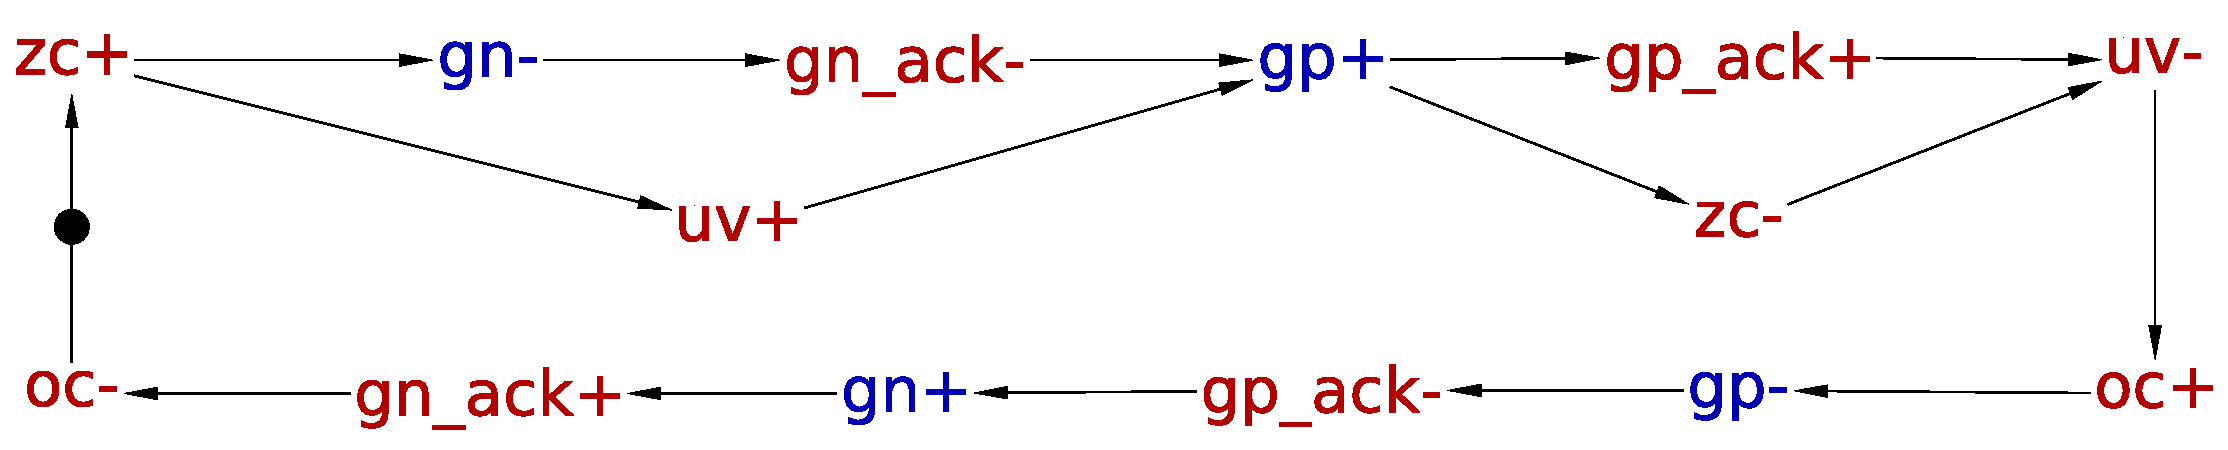
\includegraphics[scale=0.23]{Images/stg-UV_after_ZC}
\par\end{centering}

\protect\caption{\label{fig:zcEarlyScenario STG}STG for the \textsf{zcEarlyScenario}
concept.}
\end{figure}

\par\end{center}

The obtained STG for the \textsf{zcEarlyScenario} concept is shown
in Figure~\ref{fig:zcEarlyScenario STG}. We have now produced three
scenario STGs, one for each operational mode in this system. However,
we need to ensure they are correct both for the specification and
as STG models before we can combine these. 

\vspace{-2mm}



\subsection{Verification and simulation of scenarios \label{sub:Verification-and-simulation}}

\vspace{-2mm}


To be combinable by our method, the produced STGs need to have certain
properties~\cite{Cortadella}:
\begin{itemize}
\item Complete State Coding (CSC): each state of the models with different
behaviour has differing signal encodings to avoid problems during
synthesis. Note that in some cases it is possible to automatically
resolve a CSC conflict.
\item Deadlock freedom: no state is reachable from which no progress can
be made.
\item Output persistence: there are no race conditions in the STG.
\item Signal consistency: in any trace the rising and falling phases of
each signal alternate.
\end{itemize}
These properties are automatically checked in \noun{Workcraft }using
the \noun{Mpsat}~\cite{khomenko2004detecting} backend tool\noun{.
}In the event that one of these properties does not hold, unless it
can be corrected automatically, the composition of scenarios fails.
In this case a problematic concept is identified and diagnostic information
is printed out to help a designer to correct the issue.

Correctly produced scenarios may not necessarily work as the specification
suggests, and this needs to be validated before using these scenarios
in any further designs. \noun{Workcraft} features a simulation tool,
and this can be used by a designer to check that the signals can transition
according to the initial requirements. If the simulation produces
undesirable results, a designer can work to fix the error of the scenario
STG, or correct the design at the concept level. The latter is the
preferable method if this design is to be reused either as a predefined
concept, or as a scenario in another system. 

\vspace{-2mm}



\subsection{Combining scenarios }

\vspace{-2mm}


Now we have scenario STGs that have been verified to ensure they conform
to standards required of STGs, and simulated to ensure they work as
expected according to the specification. These can now be combined
to produce a full system implementation. As mentioned in Section~\ref{sub:Combination-of-scenarios},
we can combine these scenarios in multiple ways, depending on whether
there is some sort of required ordering to the way these scenarios
must run. 

For a simple buck controller there is no required order of running
these scenarios, and it is uncertain as to which scenario may be running
at any one time. Therefore, the best solution for this system is to
combine all of the scenarios in a non-deterministic fashion. The full
system implementation produced should allow for only one of these
scenarios to run at a time, but when the scenario has completed the
system should return to a state where any of the scenarios could run
again, regardless of which solution ran previously. 

\begin{figure}[t]
\begin{centering}
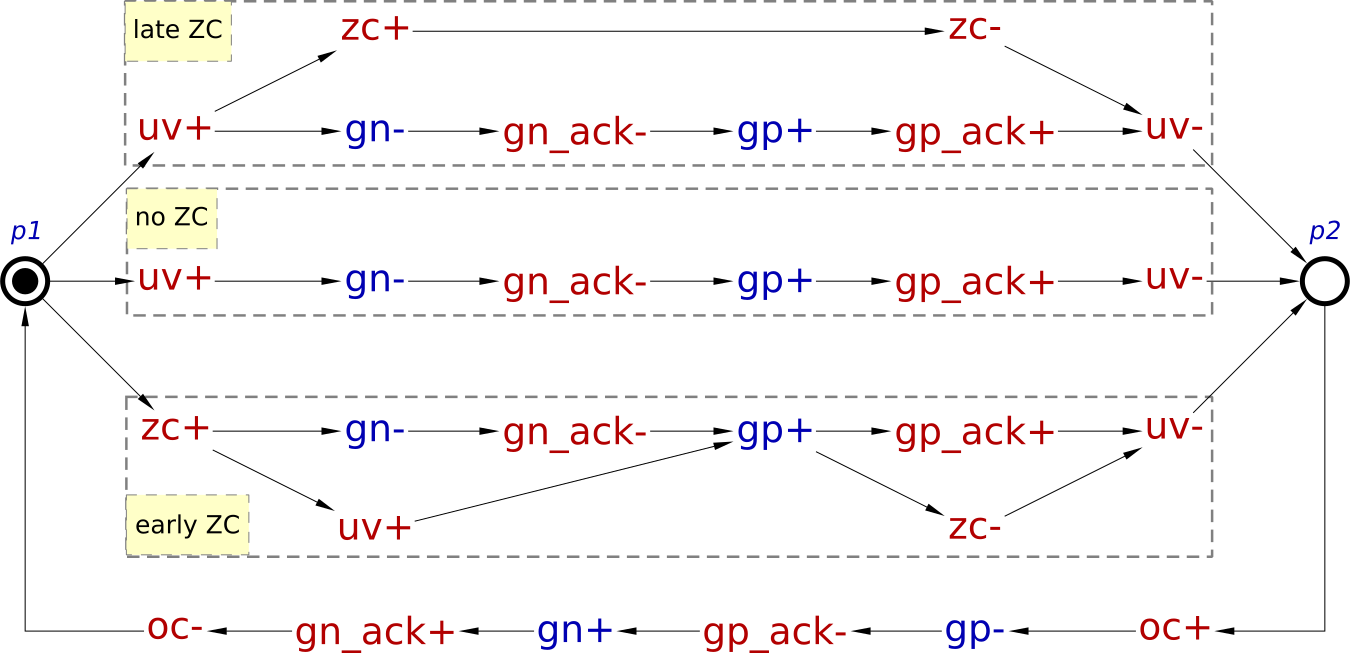
\includegraphics[scale=0.23]{Images/stg-buck}
\par\end{centering}

\begin{centering}
\protect\caption{\label{fig:buck STG}Complete STG for a buck converter.}

\par\end{centering}

\end{figure}


Figure~\ref{fig:buck STG} shows the full system specification STG
that has been produced from combining the three scenario STGs as seen
in Figures~\ref{fig:zcAbsentScenario STG},~\ref{fig:zcLateScenario STG},
and~\ref{fig:zcEarlyScenario STG}. The first most notable part of
this full system STG is that there is only one branch for over-current
correction. As mentioned above, over-current is corrected in exactly
the same way for each of these scenarios, and as such, to reduce the
complexity of the model, these can be combined into a single branch
that runs after any of the under-voltage correction branches have
run. 

There are two explicit places in this model, \textsf{p1} and \textsf{p2}.
\textsf{p1} holds a token initially, and this allows any of the scenarios
to run. This place has no control over which scenario can run, but
it only allows one of them to run at a time. The single token is consumed
by whichever scenario runs, and the lack of token in \textsf{p1} after
this stops any more scenarios running. The token is passed through
the scenario, and after under-voltage is corrected the token is passed
into \textsf{p2}. This token is then consumed by the over-current
branch, and returned to \textsf{p1}\noun{ }and this allows only one
of the scenarios to run again. 

\vspace{-3mm}



\subsection{Verification and simulation}

\vspace{-3mm}


Like with the scenario models when they have been composed, we need
to verify that this model satisfies certain properties after combination
of multiple scenarios, as any issues at this stage will cause an implementation
of the model to be wrong and this can cause the model to be unimplementable
as an SI circuit. 

The verification properties we need to satisfy are the same as for
scenarios~(see~Section~\ref{sub:Verification-and-simulation}),
and are corrected in similar ways, however the corrections can be
done within the problematic scenario, by changing, adding or removing
one or more concepts to avoid affecting any of the functionality of
the whole system, or any of the correctly functioning scenarios. 

When the full system model satisfies all of the verification properties,
we can simulate this model and check that the signals can transition
in the order we expect according to the requirements of the system.
If this is correct, we can guarantee that this model represents the
full system specification, and can now be used in the next step.

\vspace{-2.5mm}



\subsection{Synthesis of a speed-independent controller}

\vspace{-2.5mm}


A fully working model of the system is only part way to having completed
the process. The final step in this design flow is to synthesize this
model. Synthesis is the process of finding Boolean equations to calculate
the next state of the output signals based on the input signals and
the current state of the circuit~\cite{Cortadella}. We can do this
using \noun{Petrify} or \noun{Mpsat}, both of which are integrated
in \noun{Workcraft}. Passing this model through one of these tools
will produce logic equations that describe how the outputs $gp$ and
$gn$ can be produced using $uv$, $oc$, $zc$, $gp\_ack$, $gn\_ack$.
Using logic gates, we can reproduce a circuit diagram for these equations.
Figure~\ref{fig:buck Circuit} shows the logic circuit, synthesized
from this full model.

\begin{figure}[h]
\begin{centering}
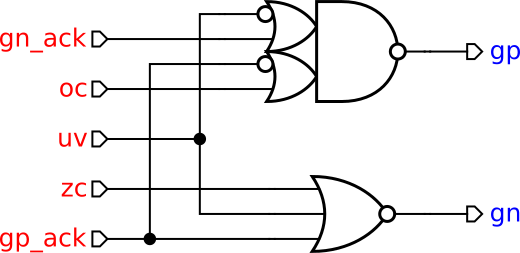
\includegraphics[scale=0.35]{Images/circuit-buck}
\par\end{centering}

\protect\caption{\label{fig:buck Circuit}Asynchronous logic gate implementation}
\end{figure}


When we have acquired a circuit design, it needs to be verified to
ensure that the logic will perform as we expected before the circuit
is fabricated. To verify this, the circuit is converted into a so-called
circuit Petri net, using a model for each logic gate and combining
them by means of read-arcs. By reachability analysis of this Petri
net one can verify that the corresponding circuit is deadlock-free,
hazard-free and conforms to the specification~\cite{2008_poliakov_async}. 



\vspace{-2mm}

\section{Related work}

\textbf{A section to include some related work, and it's comparisons with both eachother and concepts. This will be based on the lit review done earlier}

\section{Conclusions and future work}

\vspace{-2mm}


This paper shows that it is possible to design a system by splitting
it into operational modes, and describing signal interactions and
requirements of the mode in a textual format. These can then be used
to produce STGs that represent these operational modes, which can
be combined to produce a model for the full system specification.


This design method can reduce the time of designing an asynchronous
control circuit from the ground up, as well as allow reuse of components
either as part of a scenario or entire scenarios to reduce the design-time
of future projects. Composition of concepts and scenarios can help
reduce errors and save time in comparison to performing these manually.
This method can help to make asynchronous circuits more appealing
to industrial designers.

This method currently works with Signal Transition Graphs, however
it can be applied to other modelling disciplines, such as Finite State
Machines~(FSM). In some cases, a designer may wish to view a scenario
or full system model as an FSM as they can provide more information
about a system, which can help with editing finer details of system,
or when correcting errors. It would be possible to use concepts to
create scenario FSMs that can be combined to produce a full system
model in FSM form. STGs and FSMs could be interchangeable in this
respect, for example, a scenario STG could be produced, and a designer
may choose to view it as an FSM, which can be viewed by ``zooming
in'' to a section of the STG, that will expand this to show states
of the system, and possible transitions. Any edits to this can then
be used to update the overall STG. 

In addition to FSMs and STGs, we also plan to extend this design method
to support Conditional Partial Order Graphs~(CPOGs)~\cite{CPOG1}
and Parameterised Graphs~\cite{mokhov2014algebra} for modelling
asynchronous circuits. These models are also integrated into \noun{Workcraft}
as part of the \noun{Scenco} toolsuite\noun{~\cite{2015_workcraft_scenco},
}allowing circuits to be described by algebraic equations in text
form. \noun{Scenco} provides support for describing concept models
to produce scenarios and then compose scenarios to produce full system
implementations. 

In certain cases, an implementation may need to be changed based on
design parameters to produce the best result, and these may change
during run-time or after the fabrication stage. CPOGs support parameter
and run-time reconfigurability~\cite{microadapt}, hence if
design parameters change, the design does not need to be recomposed
from another list of concepts, thus saving time. For this reason,
CPOGs could work very well with this design approach. 

STGs and CPOGs both have their benefits when working with asynchronous
systems, and it will be useful to compare these two methods, to see
if either is better when designing a system from concepts, or see
if there are certain specifications where one modelling method is
better than the other. 

\vspace{-3mm}



\section*{Acknowledgements}

\vspace{-2.5mm}


The authors would like to thank the reviewers for their constructive
comments. This research is supported by EPSRC research grant `A4A:
Asynchronous design for Analogue electronics' (EP/L025507/1) and
the Royal Society research grant `Computation Alive: Design of a
Processor with Survival Instincts'.

\vspace{-2.5mm}


\bibliographystyle{unsrt}
\bibliography{publications}


\end{document}